\documentclass{article}
\usepackage[utf8]{inputenc}
\usepackage[russian]{babel}
\usepackage{graphicx}
\usepackage{amsmath}
\usepackage{breqn}
\usepackage{wrapfig}
\usepackage{float}
\usepackage{multirow}
\usepackage{caption}
\usepackage{subcaption}

\graphicspath{ {./data/images} }
\author{Александр Романов Б01-107}
\date{}
\title{3.1.1 Магнитометр}

\begin{document}
\maketitle
\section{Введение}
\subsection{Цель работы}
Определить горизонтальную составляющую магнитного поля Земли и установить количественное соотношение между
единицами электрического тока в системах СИ и СГС.
\subsection{В работе используются}
Магнитометр, осветитель со шкалой, источ­ник питания, вольтметр, электромагнитный переключатель, конденсатор,
намагниченный стержень, прибор для определения периода крутильных
колебаний, секундомер, рулетка, штангенциркуль.
\begin{figure}[h]
    \centering
    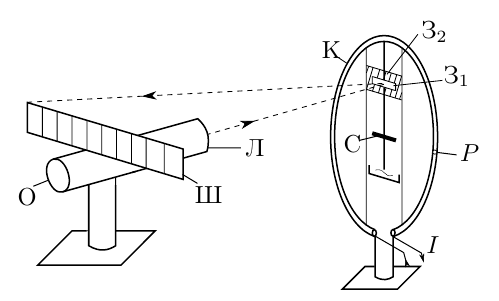
\includegraphics[width=0.6\textwidth]{scheme.png}
    \caption{Схема экспериментальной установки}
    \label{fig:sheme}
\end{figure}

\begin{figure}[h]
    \centering
    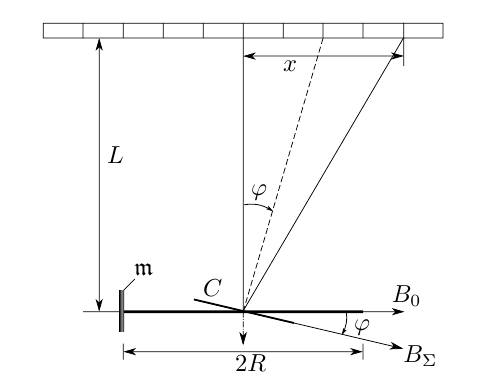
\includegraphics[width=0.6\textwidth]{angles.png}
    \caption{Схема измерения угла отклонения магнитной стрелки}
    \label{fig:sheme}
\end{figure}

\section{Работа}
\subsection{Измерение угла отклонения магнитной стрелки в поле намагниченного стержня}
Включим осветитель и получим на экране 2 чётких световых зайчика. Плавным поворотом кольца К вокруг вертикальной
оси совместим эти зайчики. В отверстие P вставим намагниченный стержень и измерим смещение подвижного зайчика \(x_1\):
\[ x_1 = 5.5\; cm \]
Поменяем ориентацию стержня и измерим отклонение стержня в другую сторону:
\[ x_1 = 5.5\; cm \]
Отклонения идеально совпадают.

Измерим расстояние \(L\) от шкалы до зеркала:
\[ L = 81\; cm \]

\subsection{Измерения периода колебания намагниченного стержня в поле Земли}

Поставим стеклянный сосуд вблизи магнитометра и опустим на дно намагниченный стержень, привязанный за середину.

Измерим период колебаний стержня в поле Земли:
\[ T = 7.3\; s\]

Измерим параметры стержня:
\begin{table}[H]
    \centering
    \begin{tabular}{|c|c|c|}
    \hline
    \(l,\; cm\) & \(d, \; cm\) & \(m, g\) \\\hline
    4 & 0.5 & 5.9 \\\hline        
    \end{tabular}
\end{table}

Радиус кольца:
\[ R = 20\; cm \]

Рассчитаем величину горизонтальной составляющей магнитного поля Земли \(B_0\) по формуле:
\[ B_0 = \frac{2\pi}{TR}\sqrt{\frac{\mu_0JL}{2\pi Rx_1}} = 0.146\cdot10^{-4}\; T \]

\subsection{Измерение электродинамической постоянной}

\section{Выводы}
\end{document}